%!TEX root = ../thesis.tex
本章では,オープンプラットフォームのロボットアームの要求仕様を決定していく.行わせる作業を設定し,設定した作業と既存のオフィスロボットの調査を基に要求仕様をまとめていく.
\section{作業の設定}
本研究では,オフィス環境におけるロボットアームの作業としてデスクの片づけを設定した.オフィス環境で想定される作業は多岐にわたるが,基本的には台車移動とピック&プレイス作業を組み合わせたものが大半を占める.これは既存のオフィスロボットがどのような作業を対象にしているかを調査した結果である.文献や動画から78の作業内容を抽出し,そのうち66件(約85%)が台車移動とピック&プレイス作業を組み合わせたものであった.本研究で開発するアームは,将来的にオフィスロボットのプラットフォームとなることを期待しているため,最初のステップとしてこの作業を設定した.作業環境のイメージ図を図\ref{fig:range}に示す.図のように,部屋の中にある机の上に対象物と箱を配置し,全ての対象物を箱の中に入れるというシンプルな作業である.対象物と箱は机の縁から50cm以内の範囲に設置する.また,対象物に関しても既存のオフィスロボットが扱っているものを調査し決定した.調査結果を表に示す.最も多かったのは衣類などの柔軟な物体であり,次いでボトルなどの円柱型の物体が多かった.今回はこれらの中からボトルとタオルを対象物として設定した.調査した作業内で重量の大きい対象物を把持している作業は確認できず,多くは軽量な物体を把持していた.そのため,対象物の重量は500g以下とする.片づける箱のサイズは,高さ20cmとする.
\begin{figure}[h]
  \centering
  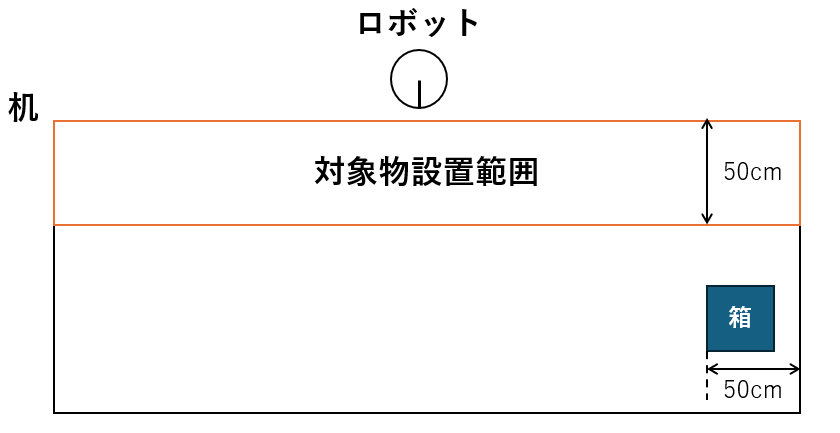
\includegraphics[width=10cm]{images/range.png}
  \caption{対象物と箱の設置範囲}
  \label{fig:range}
\end{figure}
\begin{figure}[h]
  \centering
  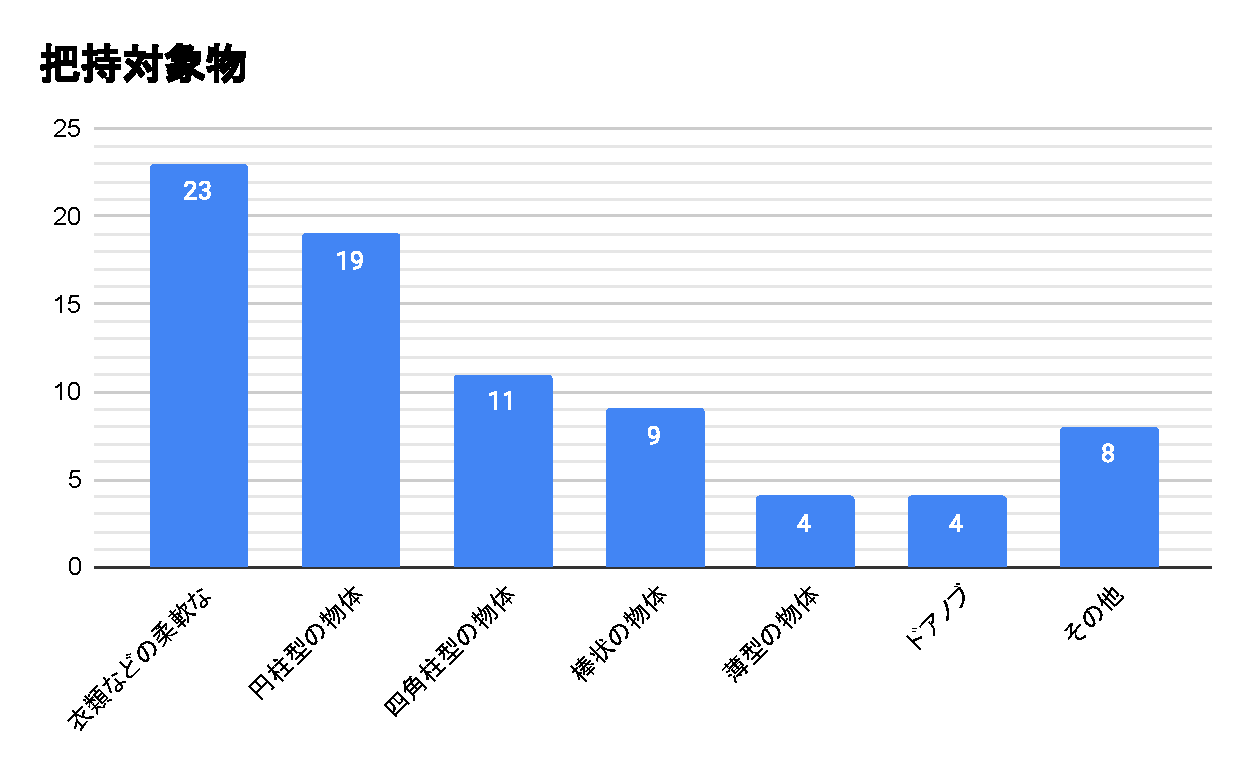
\includegraphics[width=10cm]{images/handget.pdf}
  \caption{既存のオフィスロボットが扱っている対象物}
  \label{fig:handget}
\end{figure}
\newpage